\documentclass[a4paper,11pt,oneside]{book}

\usepackage[english]{babel}
\usepackage[showframe=false]{geometry}
\usepackage[usenames,dvipsnames]{xcolor}
\usepackage[utf8]{inputenc}
\usepackage[T1]{fontenc}
\usepackage{changepage}
\usepackage[]{algorithm2e}
\usepackage{amssymb}
\usepackage{amsmath}
\usepackage{graphicx}
\usepackage{listings}
\usepackage{verbatimbox}
\usepackage{ulem}
\usepackage{fancyvrb}
\usepackage{float}
\usepackage{hyperref}
\usepackage[parfill]{parskip}
\usepackage{tikz}
\usepackage{pdflscape}
\usepackage{minted}
\usepackage{titlesec}
\usepackage{titleps}
\usepackage{lastpage}
\usepackage{fancyhdr}
\usepackage{etoolbox}
%Following overwrites the page style for chapters
\patchcmd{\chapter}{\thispagestyle{plain}}{\thispagestyle{ruledChapter}}{}{}

%New page style for chapters
\newpagestyle{ruledChapter}{
	\setfoot{}{\thepage\ of \pageref{LastPage}}{}
	\footrule
	\renewcommand\makefootrule{\color{black}\rule[\baselineskip]{\linewidth}{0.4pt}}
}
%New page style for rest
\newpagestyle{ruled}{
	\sethead{\raggedright \chaptername\ \thechapter :\ \chaptertitle}{}{}
	\headrule
	\setfoot{}{\thepage\ of \pageref{LastPage}}{}
	\footrule
	\renewcommand\makeheadrule{\color{black}\rule[-.3\baselineskip]{\linewidth}{0.4pt}}
	\renewcommand\makefootrule{\color{black}\rule[\baselineskip]{\linewidth}{0.4pt}}
}

\expandafter\def\csname PY@tok@err\endcsname{}
\newcommand{\HRule}{\rule{\linewidth}{0.5mm}}
\newcommand{\specialcell}[2][c]{%
  \begin{tabular}[#1]{@{}c@{}}#2\end{tabular}}

\addtocontents{toc}{\protect\thispagestyle{empty}}

\title{}
\author{}
\date{} 

\begin{document}
\begin{titlepage}
\begin{center}

%-----------------------------------------------------------------
%							FRONTPAGE
%-----------------------------------------------------------------
\thispagestyle{empty}

\includegraphics[width=0.55\textwidth]{logo.pdf}\\[1cm]    
\textsc{\Large DM818 Assignment 1}\\[0.5cm]

% Title
\begin{Huge}
\textbf{Matrix Multiplication}
\end{Huge}

\vspace{4cm}

% Author and supervisor
\begin{minipage}{1\textwidth}
\begin{center}
\emph{}\\

Dan \textsc{Sebastian Thrane}\\
\verb!<dathr12@student.sdu.dk>!\\

Lars \textsc{Thomasen}\\
\verb!<latho12@student.sdu.dk>!\\

\end{center}
\end{minipage}
\begin{minipage}{0.4\textwidth}
\end{minipage}

\vfill
\begin{tabular}{ll}
    Aligned SSE: yes \\
    Unaligned SSE: no \\
\end{tabular}
\vfill

% Bottom of the page
{\large Fall 2015}\\

\end{center}
\end{titlepage}

%-----------------------------------------------------------------
%							   TOC
%-----------------------------------------------------------------
\renewcommand{\contentsname}{Table of Contents}
\tableofcontents
\thispagestyle{empty}

%-----------------------------------------------------------------
%						  ACTUAL REPORT
%-----------------------------------------------------------------
\pagestyle{ruled}
\chapter{Introduction}
\setcounter{section}{1}
This report covers the task of optimizing matrix multiplication on a single core. For this task access to the NERSC cluster has been supplied, thus majority of the performance tweaking was been focused for this. Code for running on the SDU Imada terminal room has also been developed, however values are not tweaked as well there.

\section{Work load}
This assignment has been done in a group of two, following pair programming principles. Thus the work load has been evenly divided, majority of the work load being converting theoretical theories into actual code and doing things correctly.


\chapter{Optimizations}
% The optimizations used or attempted
% The results of those optimizations
\section{Overview}
This section gives a short overview of optimization ideas followed/used. Further details are covered in the following subsections.

\begin{itemize}
\item Blocking Matrix Multiplication.
\item Packing data.
\item SIMD/SSE instructions.
\item Loop unrolling.
\item Compiler flags.
\end{itemize}

\subsection{Blocking algorithm}
Following the supplied code for the blocking algorithm, this was expanded upon following the \emph{Goto, K., and van de Geijn, R. A. 2008. Anatomy of High-Performance Matrix Multiplication} article.

Initially the blocking method was changed to block in slithers rather than square blocks, as illustrated below. This should take advantage of better data locality, since (atleast for the B matrix) more data would come contiguously, before jumping to the next column.

% TODO: insert awesome image.

This blocking method was later reverted due to performance issues for very large matrices, where for high K values the cache would be filled and start swapping out needed data. This can clearly be seen in the graph below as performance decreases the higher the size of the matrix. This was unavoidable as the slithers always had K length, and even blocking with low values would eventually contain too many elements.

\begin{figure}
  \centering
  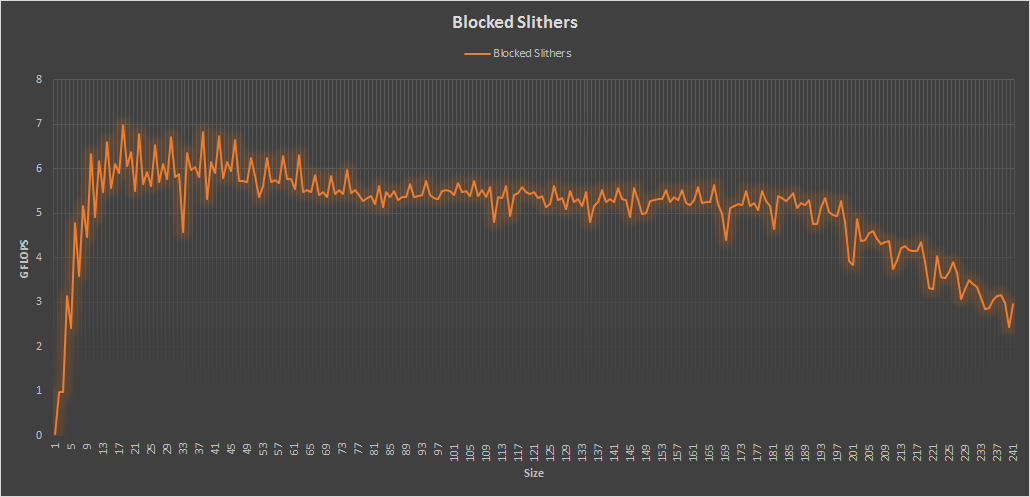
\includegraphics[width=0.9\linewidth]{graph-blocked-downcurve.png}
  \caption{Blocked slithers performance for sizes 1 to 241 with interval of 4. Block value at an absolute minimum.}
  \centering
  \label{fig:sub1}
\end{figure}

The reverted state would be blocked in square matrices with values for N, M and K being the BLOCK\_SIZE, except for the fringe cases.

% TODO: Should we go into explaining what fringe cases is here, or is this considered trivial? Should probably ask Daniel about this.

\subsection{Packing data}
In order to improve data locality, and take advantage of loading SSE instructions, data had to be re-arranged. This required new auxiliary arrays for the packed data, aligning it for 16bytes (the size of a double). The cost of packing is almost identical to loading in the data in the first place, thus this cost is quickly recovered later on.

The theory behind packing data is very simple, and it is much more interesting when to do this in order to exploit having the data available later on. 

We first pack the entire B matrix, and then pack the A matrix in slivers of size $mc$. The order of this packaging ensures that the relevant $mc$ rows of the A matrix is always in memory along with most, if not all, of the B matrix too. By packing slivers of the A matrix we are able to increase the block size in general and still keep it all in memory. The idea behind this is that when we load in the next sliver of A, the least recently used data will be the old A matrix. %TODO: I need to rewrite this section.

\subsection{SIMD instructions}
Single instruction, multiple data (SIMD) is a form of parallelism with multiple processing elements that perform the same operation on multiple data simultaneously. This means that we can multiply several numbers (2 doubles in this case) with each other at the same time. This method requires the data to be aligned when loading it, which is covered in the packing process described previously.

By using SIMD instructions, we are able to cut the K iterations in half by doing two iterations at the same time with no additional cost. %true?

This requires padding the K elements to an equal number of elements, a trivial but important step to keep the calculations correct.

\subsection{Loop Unrolling}
% TODO: I need to read up a slight bit on exactly how this works, but the gist of it is correct. (What is the difference between hardware pipelning and software pipelining exactly?).
In order to exploit pipelining, loop unrolling has been performed in the inner-most matrix multiplication. By loop unrolling the actual multiplication of the elements, the hardware is able to do several computations at once, before having to wait for the multiplication to finish and continuing the loop.

% Insert code example here?

%Padding:
In order to perform loop unrolling, padding was initially used such that fringe cases would not cause the program to access data outside of the arrays. This padding was done by simply putting the value 0 into the additional elements accessed, as this would not change the correctness of the matrix multiplication.

This padding resulted in performance dips for matrix sizes which did not fit into a multiplicative of the unrolled size. This behaviour is clearly seen in the figure below. The explanation for this lies in the added calculations of the zeroes, along with using an auxiliary array for the result matrix.

The auxiliary array was necessary as padding the result matrix was infeasible when writing to values outside its array. This writing to a temp array and moving only the relevant entries was the best solution we could come up with.

\begin{figure}
  \centering
  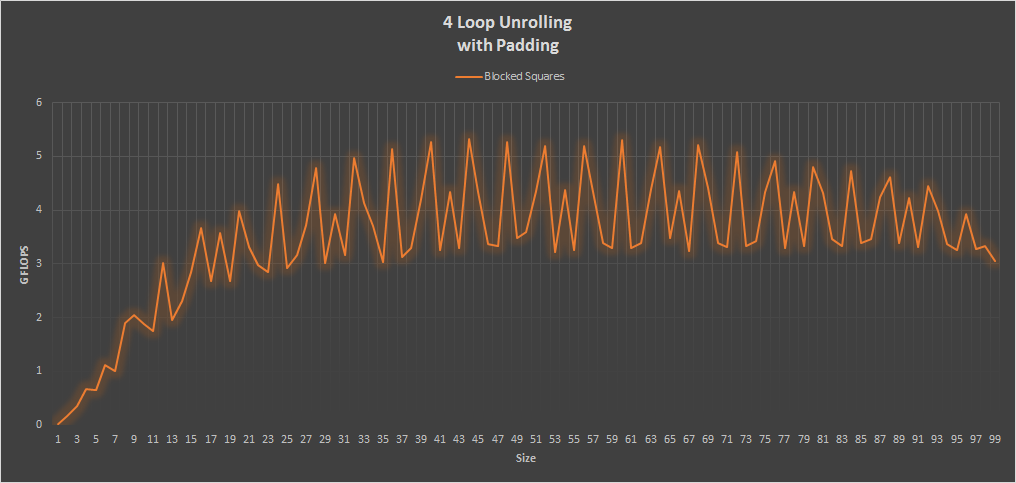
\includegraphics[width=0.9\linewidth]{graph-blocked-padding.png}
  \caption{Unrolling the access to the B matrix with 4, using padding to handle fringe cases.}
  \centering
  \label{fig:sub1}
\end{figure}

This solution was improved upon by doing an early check of the actual block size, and then calling the method best fitted for that block size, such that loop unrolling could be maximized.

\chapter{Performance}
% How the same kernel performs on a different hardware platform (and a small discussion of that)
% TODO: Need to test this, Hooper VS Imada, and how the different architectures are (since this is the primary reason for variation).

\section{Hopper}
\subsection{Graphs}
% A figure fhat shows the performance similar than the figure above, but using all matrix sizes 2, 3, 4, ..., 769 for a single processor core of NERSC Hopper cluster (y-axis should say percentage of peak performace).
\subsection{Odd behaviours}
% The reason for any odd behavior (e.g., dips) in performance.

\subsection{Peak performance}
% Explain how you determined the peak performace, and again, the y-axis should say percentage of peak performance.


\section{Imada machines}
\subsection{Graphs}
% A figure fhat shows the performace similar than the figure above, but using all matrix sizes 2, 3, 4, ..., 769 for a single processor of another system of your choice (using the same kernel). 

\chapter{Conclusion}
% A short recap of what we achieved and the results.


%-----------------------------------------------------------------
%						     APPENDIX
%-----------------------------------------------------------------
%\newpage
%\newgeometry{left=2.5cm,right=2.5cm}
%\chapter{Appendix}
%\section{Source code}

\end{document}
